\subsection*{Проблема градиентного спуска}

Мы уже показали, что идеальные разбиения, зачастую, являются переобученными деревьями, но что если попытаться найти такое разбиение, которое
\begin{itemize}
    \item Идеально классифицирует выборку;
    \item Не переобучено?
\end{itemize}

И тут ситуация, крайне похожая на линейные классификаторы: поиск такого разбиения можно осуществить только перебором, что опять является \texttt{NP}"=полной задачей.

А теперь обсудим другой вопрос "--- а что там с градиентым спуском? На самом деле, не очень похоже на то, что тут можно как"=то адекватно его применить. В первом приближении это действительно так, но стоит лишь взглянуть на задачу под другим углом.

Давайте построим следующий жадный алгоритм, который позволит с нуля строить деревья:
\begin{algorithm}
\begin{tabbing}
\hspace{0.3cm} \= \hspace{0.6cm} \= \hspace{0.9cm} \= \kill
FitNode($m$, $RM$): \\
\> \textbf{if} выполнен критерий остановы: \textbf{then} \\
\> \> находим $cm$ \\
\> \> объявляем вершину листовой \\
\> \> \textbf{return} \\
\> \textbf{end}
\end{tabbing}
\end{algorithm}

Критерий остановы (в контексте нашей лекции) "--- условие, при соблюдении которого мы прекращаем строить дерево, считая, что оптимальное уже достигнуто. Например:
\begin{itemize}
    \item Если достигли максимальной глубины;
    \item Если количество объектов в узле меньше некоторого порога;
    \item \dots
\end{itemize}

Если же критерий остановы не выполнен, то мы хотим получить какое"=то разбиение для предиката. Будем рассматривать для предиката 
\[
[x_j < t]
\]

\newpage
Будем искать оптимальные порог и признаки такого предиката следующим образом:
\[
j_*, t_* = \arg\max_{j, t} ~ Q (R_m, j, t)
\]

Появляется масса вопросов:
\begin{itemize}
    \item Что такое $Q$? Как его искать?
    \item Как найти прогноз в листовой вершине?
    \item Какой критерий остановы подойдёт?
    \item Как находить оптимальные пороги и признаки?
\end{itemize}

\subsubsection*{Критерий остановы}

Проще всего будет разобраться с критерием остановы. На самом деле, выше уже приведены такие критерии, которые подойдут. Можно и придумать свои, но главное, чтобы они были осмысленными.

\subsubsection*{Оптимальные пороги и признаки}

Тут уже немного сложнее. Для начала важно понять суть предикатов: формально, мы задаём нашей выборке какой"=то <<вопрос>>, по результатам которого разделяем выборку на части. И текущая задача заклюается в том, чтобы эти <<вопросы>> были как можно более эффективными. Но что значит эффективными?

Представьте, что Вы играете в игру "20 вопросов", в которой один человек загадывает личность, а второй должен попытаться отгадать её, задавая только вопросы с ответами "Да"/"Нет". И здесь, аналогично, отгадывающий вынужден корректно подбирать вопросы. Например, если человек безуспешно сразу попытается отгадать, то у него останется ещё 8 миллиардов вариантов того, кто это может быть. Однако если спросить пол, то это отсечёт уже около половины кандидатов.

\newpage
За этими рассуждениями стоит крайне важное понятие во многих технических сферах "--- \textit{энтропия} (степень хаоса).
Формально, она определяется как
\[
S = - \sum_{i=1}^N p_i \log_2 p_i
\]

где $p_i$ "--- вероятность появления $i$"=го класса в рассматриваемом множестве, $N$ "--- общее число классов. Используется соглашение о том, что $0 \log_2 0 = 0$.

Энтропия (Шеннона) принимает значения $[0, 1]$, где 
\begin{itemize}
    \item $0 \Rightarrow $ в узле наблюдается равномерное распределение (полный хаос, абсолютно случайные точки);
    \item $1 \Rightarrow $ вырожденное распределение (все объекты принадлежат одному классу, нет никакого хаоса).
\end{itemize}

Давайте перейдём к практическому примеру.
\begin{figure}[H]
    \centering
    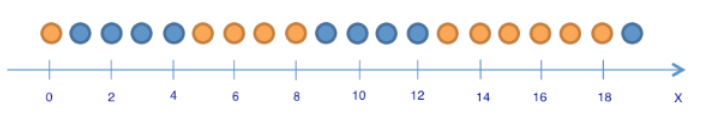
\includegraphics[width=0.75\linewidth]{img/entropy1.png}
\end{figure}

Здесь у нас есть 20 шариков, из которых 9 синих и 11 оранжевых.
Соответсвенно, 
\[
p_1 = \frac{9}{20}, p_2 = \frac{11}{20}
\]

Посчитаем текущую энтропию:
\[
S_0= - \frac{9}{20} \log_2 \frac{9}{20} - \frac{11}{20} \log_2 \frac{11}{20} \approx 1
\]

Энтропия даёт понять, что происходит примерно хаос "--- это можно заметить и визуально.

\newpage
Давайте вручную сделаем предикат. Скажем, разобъём шарики на 2 лагеря по признаку $[x \le 12]$:
\begin{figure}[H]
    \centering
    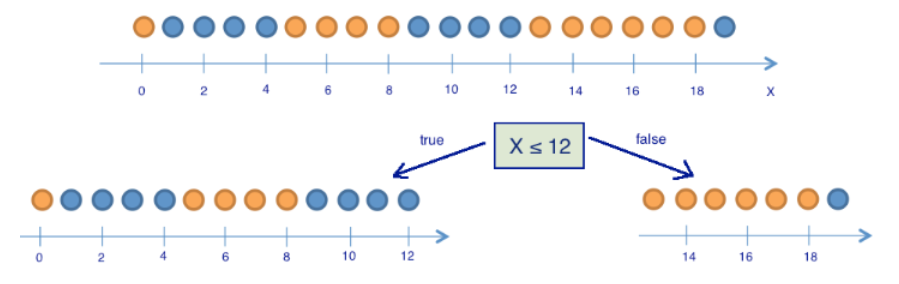
\includegraphics[width=0.75\linewidth]{img/entropy2.png}
\end{figure}

В каждой из подвыборок посчитаем энтропию. Начнём с левой:
\[
S_1 = - \frac{5}{13} \log_2 \frac{5}{13} - \frac{8}{13}\log_2 \frac{8}{13} \approx 0.96
\]
А теперь для правой:
\[
S_2 = - \frac{1}{7}\log_2 \frac{1}{7} - \frac{6}{7}\log_2\frac{6}{7} \approx 0.6
\]

Особенно для правого случая видим, что энтропия заметно снизилась, что заметно как и численно, так и визуально.

Формально, понижение энтропии ещё называют \textit{приростом информации}, однако о подробностях этого процесса мы поговорим на следующем занятии.